\fontsize{14}{15}\selectfont
\section{Caso de estudio}
\lipsum[1]\\
\section{Planteamiento del Problema}
\lipsum[1]\\
\section{Objetivos}
\subsection{Objetivo General}
\begin{itemize}
	\item Determinar la condición física de los alumnos de la Carrera de Geología de la UCN.
\end{itemize}
\subsection{Objetivos Específicos}
\begin{enumerate}
	\item Identificar los lineamientos o posibles fallas en el área de estudio. 
	\item Establecer marcadores morfológicos para la conocer su cinemática.
	\item Determinar tipo de movimiento y/o características tienen los rasgos estructurales del área.
\end{enumerate}
\section{Ubicación del área de estudio}
El área de captación por las técnicas ocupadas (InSAR y GPS), pueden abarcar aún más territorio hacia el norte, sur, y este de la península, llegando a ser cerca de 27.000 km$^2$ (Figura \ref{ilustracion1}).\\
\begin{figure}[hb]
	\centering
	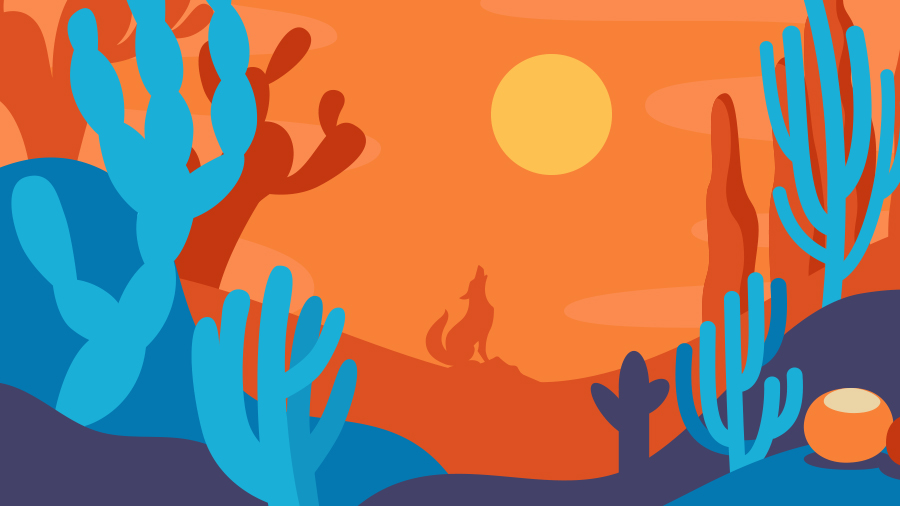
\includegraphics[scale=0.4]{figure1.jpg} %Change the figure name 
	\setstretch{1} %Interlineado 1
	\captionsetup{labelsep=period, labelfont=bf}
	\caption[Ilustración zorro en desierto]{\blindtext[1]} %[Se muestra en el índice]{Se muestra en el pie de figura}
	\label{ilustracion1}
\end{figure}



\section{Data y Metodología}
\lipsum[1]